\documentclass[12pt, titlepage]{report}
\usepackage[spanish]{babel}
\usepackage[none]{hyphenat}
\usepackage[margin=3cm]{geometry}
\usepackage{graphicx}
\usepackage{subcaption}
\usepackage[hidelinks]{hyperref}
\usepackage{parskip}

\sloppy
\setlength{\parindent}{0cm}
\graphicspath{{img/}}
\decimalpoint
\hypersetup{colorlinks=true, urlcolor=blue}
\urlstyle{same}

\begin{document}
    \begin{titlepage}
        \begin{center}
            \begin{figure}[ht]
                \centering
                \begin{subfigure}[r]{0.15\textwidth}
                    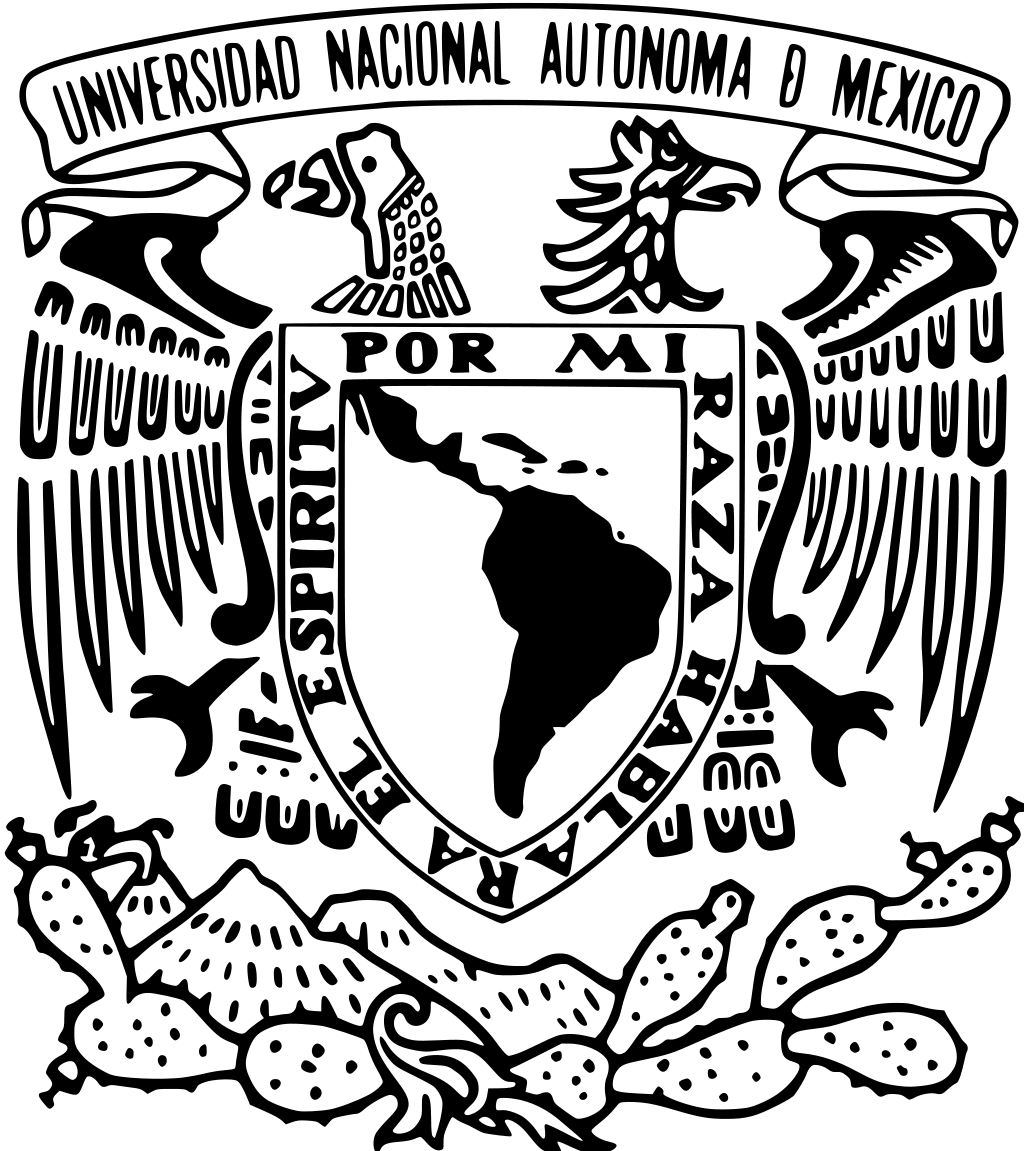
\includegraphics[width=\textwidth]{Escudo_UNAM.png} 
                \end{subfigure} \hspace{9cm} 
                \begin{subfigure}[l]{0.15\textwidth}
                    
\includegraphics[width=\textwidth]{Escudo_FI.png}
                \end{subfigure} 
            \end{figure}

            \large \textbf{UNIVERSDAD NACIONAL AUTÓNOMA DE MÉXICO\\}
            \large \textbf{\\FACULTAD DE INGENIERÍA\\} 
            \hfill \break
            \large Laboratorio de Mecánica\\
            \Large \textbf{\\Práctica No. 5\\}
            \large Movimiento rectilíneo uniformemente variado\\
            \Large \textbf{\\Nombre del profesor\\}
            \large Lorenzo O. Miranda Cordero\\
            \Large \textbf{\\Grupo 8\\}
            \Large \textbf{\\Brigada \\}
            \Large \textbf{\\Integrantes:\\}
            \Large Acosta Porcayo Alan Omar\\2. \\3. \\4. \\
        \end{center}
        \begin{flushright}
            \Large \textbf{Semestre 2023-2}
        \end{flushright}
    \end{titlepage}

    \section*{Introducción}
    Se llama movimiento rectilíneo uniformemente variado a aquel movimiento rectilíneo de una partícula en el cual el valor de la aceleración es constante.

    Este tipo de movimiento se presenta en la caída libre, el tiro vertical y en el movimiento de cuerpos bajando por un plano inclinado.

    Es relativamente fácil de reproducir en el laboratorio, y es por ello que frecuentemente se le escoge para verificar el comportamiento cinemático de los cuerpos con dicho movimiento.

    La fuerza de fricción seca es una fuerza tangencial entre dos superficies que tiende a oponerse al movimiento relativo de dichas superficies.

    El comportamiento de esta fuerza lo establecen relaciones empíricas determinadas por las leyes de Coulomb-Morin, las cuales no constituyen leyes físicas científicas fundamentales como las leyes de Newton.

    El coeficiente de fricción cinética depende principalmente de la naturaleza de las superficies en contacto, es relativamente grande cuando son muy ásperas y pequeño cuando están razonablemente pulidas; además, varía algo con la velocidad relativa y es más o menos independiente del área en contacto, aunque para efectos prácticos se le considera invariante con respecto a la rapidez de movimiento.

    La determinación del coeficiente de fricción cinética de manera experimental es muy importante para la comprensión y el análisis de los fenómenos en los que se presenta. 

    \section*{Objetivos}
    \begin{enumerate}
        \item Determinar la magnitud de la aceleración de un carro que se desplaza de forma rectilínea sobre un plano inclinado, mediante la caracterización de la variación de su posición con respecto al tiempo, con el empleo de \textit{Mathematica}. 
        \item Calcular a partir del valor de la aceleración, la constante $g$ del campo gravitatorio terrestre, conocido el ángulo de inclinación del plano de movimiento. 
        \item Con base en la caracterización de la variación de la posición de un bloque con respecto al tiempo que se mueve sobre un plano inclinado con dos coeficientes de fricción diferentes, obtener el valor del coeficiente de fricción cinética que se establece entre las superficies en contacto. 
        \item Trazar con \textit{Mathematica} o algún otro software preferentemente matemático, las gráficas posición vs. tiempo, rapidez vs. tiempo, aceleración vs. tiempo y rapidez vs. posición, que representan el comportamiento de los movimientos estudiados en esta práctica. 
    \end{enumerate}

    \section*{Primer Experimento}
    El primer experimento consistió en tomar las mediciones de posición vs. tiempo de un carro dinámico que se desplaza por una rampa de aluminio con 10° de inclinación. Para registrar los datos se utilizó un sensor de movimiento, la interfaz \textit{Science Workshop 750}, una computadora personal (PC) y el software \textit{PASCO Capstone}.

    \begin{figure}[ht]
        \centering
        \setcounter{figure}{0}
        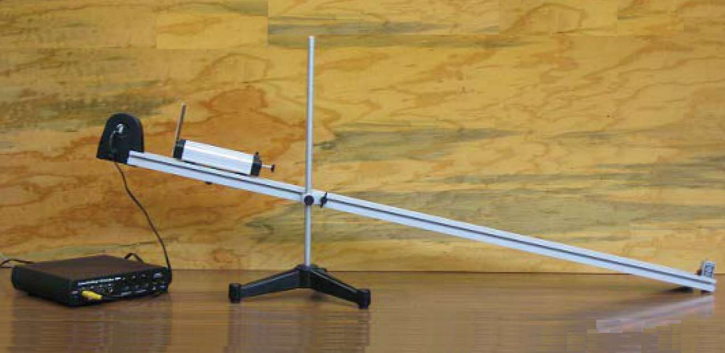
\includegraphics[width=0.5\textwidth]{Rampa_Exp1.png}
        \caption{Configuración del primer experimento}
    \end{figure}

    Para registrar los datos por medio del software \textit{PASCO Capstone} fue necesario configurar el sensor de movimiento: la frecuencia de muestreo se cambió a 50 Hz y el tipo de registro se configuró en basado en tiempo con una duración de 2 segundos. 

    Para la toma de datos fue necesaria la sincronización de por lo menos tres miembros de la brigada. Un miembro se encargó de presionar el botón de \textit{Registro} en la PC, otro miembro sostenía al carro en la posición inicial y un tercer miembro se colocó al final de la rampa para prevenir que el carro se dañara.

    Tras cada medición se exportaron los datos en una memoria USB en formato de texto plano (.txt). Los datos obtenidos tienen el siguiente formato:

    \begin{figure}[ht]
        \centering
        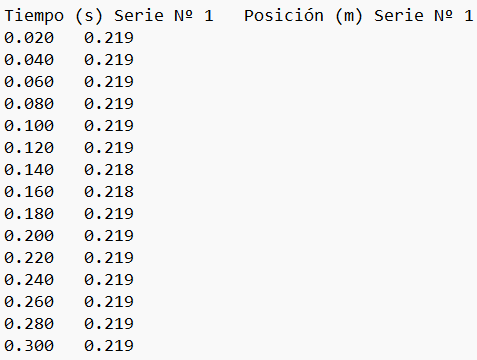
\includegraphics[width=0.5\textwidth]{Formato_Datos.png}
        \caption{Registro de datos}
    \end{figure}
    
    

    \section*{Segundo Experimento}


    \newpage
    \section*{Conclusiones}

    \section*{Bibliografía}
    Práctica 5. Movimiento rectilíneo uniformemente variado. Manual de Prácticas del Laboratorio de Mecánica, División de Ciencias Básica, 2022. \url{https://bit.ly/43A70I3}
    
\end{document}